Multiple choice section. All points are for choosing the correct answer(s). No justification is needed.
\begin{questions} 



\question[3] Select a polynomial of smallest degree with roots of $6$, $\sqrt{7}$, a repeated root of $-3$ with a multiplicity of $2$, 
and a leading coefficient of $-5$.

\begin{checkboxes}
    \choice $(x-6)(x-\sqrt{7})(x+3)^2 $
    \choice $-5(x-6)(x-\sqrt{7})(x+3)^2 $
    \choice $(x+6)(x+\sqrt{7})(x-3)^2(x-5) $
    \choice $-5(x+6)(x+\sqrt{7})(x-3)^2 $
    \choice None of the above.
\end{checkboxes}

\question[3] You run a business teaching aspiring didgeridoo players. Let $x$ be the number of hours you spend teaching your students. If the equation for your profit (in dollars) is given by
\[ P(x) = 28 x-35\]
What is the rate of change and what does it represent in this equation?
\begin{checkboxes}
    \choice You earn \$28 dollars per hour teaching.
    \choice You make 28 didgeridoos per hour.
    \choice You lose \$35 dollars per hour teaching.
    \choice $x=\dfrac{5}{4}$
    \choice None of the above.
\end{checkboxes}

\question[3] Consider a polynomial
\[P(x) = ax^7+3x^5-4x+12\]
You do not know $a$, but you know as $x\to-\infty$ $P(x)\to+\infty$. What else do you know?
\begin{checkboxes}
    \choice As $x\to+\infty$\, $P(x)\to+\infty$
    \choice $P(x)$ has seven rational roots.
    \choice As $x\to+\infty$\, $P(x)\to-\infty$
    \choice $P(x)$ has seven real roots.
    \choice None of the above.
\end{checkboxes}
\newpage
\question[3] Given the graph of $f(x)=2^x$ below, select the correct graph of $g(x)=\dfrac{1}{4}2^{-x}+1$  

\begin{center}
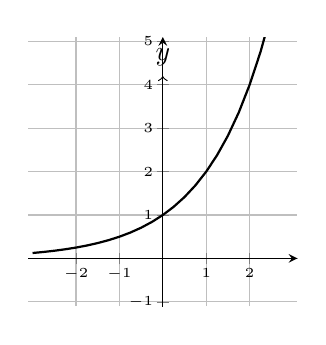
\begin{tikzpicture}%[domain=-4:4]
    \begin{axis}[
    grid=major,
    axis x line = middle,
    axis y line = middle,
        yticklabel style = {font=\tiny,xshift=0.5ex},
        xticklabel style = {font=\tiny,yshift=0.5ex},
    %scale only axis=true,
    width=5 cm,
    height=5 cm,
    xtick={-2,-1,0,1,2},
    ytick={-2,-1,0,1,2,3,4,5},
    xmin=-3.1,
    xmax=3.1,
    ymin=-1.1,
    ymax=5.1,
    ]
  %\draw[very thin,color=gray] (-2.9,-2.1) grid (2.9,2.9);

  \draw[->] (-4.2,0) -- (4.2,0) node[right] {$x$};
  \draw[->] (0,-1.2) -- (0,4.2) node[above] {$y$};

  \draw[thick, domain=-3:3]    plot (\x,2^\x) ;%            node[right] {$f(x) =x$};
  % \x r means to convert '\x' from degrees to _r_adians:
  %\draw[thick, domain=-1:2]   plot (\x,2*\x) ;%   node[right] {$f(x) = \sin x$};
  %\draw[color=orange] plot (\x,{0.05*exp(\x)}) node[right] {$f(x) = \frac{1}{20} \mathrm e^x$};
  \end{axis}
\end{tikzpicture}
\end{center}

\begin{multicols}{2}
    

\begin{checkboxes}
    \choice \phantom{a}\vspace{-.7cm}
    
    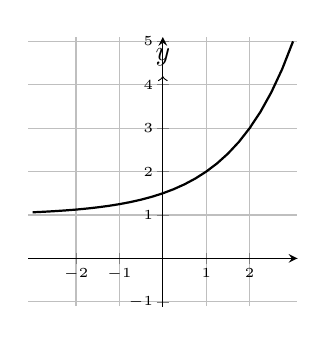
\begin{tikzpicture}%[domain=-4:4]
    \begin{axis}[
    grid=major,
    axis x line = middle,
    axis y line = middle,
        yticklabel style = {font=\tiny,xshift=0.5ex},
        xticklabel style = {font=\tiny,yshift=0.5ex},
    %scale only axis=true,
    width=5 cm,
    height=5 cm,
    xtick={-2,-1,0,1,2},
    ytick={-2,-1,0,1,2,3,4,5},
    xmin=-3.1,
    xmax=3.1,
    ymin=-1.1,
    ymax=5.1,
    ]
  %\draw[very thin,color=gray] (-2.9,-2.1) grid (2.9,2.9);

  \draw[->] (-4.2,0) -- (4.2,0) node[right] {$x$};
  \draw[->] (0,-1.2) -- (0,4.2) node[above] {$y$};

  \draw[thick, domain=-3:3]    plot (\x,0.5*2^\x+1) ;%            node[right] {$f(x) =x$};
  % \x r means to convert '\x' from degrees to _r_adians:
  %\draw[thick, domain=-1:2]   plot (\x,2*\x) ;%   node[right] {$f(x) = \sin x$};
  %\draw[color=orange] plot (\x,{0.05*exp(\x)}) node[right] {$f(x) = \frac{1}{20} \mathrm e^x$};
  \end{axis}
\end{tikzpicture}

\choice \phantom{a}\vspace{-.7cm}
    
    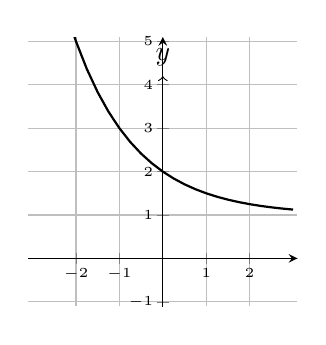
\begin{tikzpicture}%[domain=-4:4]
    \begin{axis}[
    grid=major,
    axis x line = middle,
    axis y line = middle,
        yticklabel style = {font=\tiny,xshift=0.5ex},
        xticklabel style = {font=\tiny,yshift=0.5ex},
    %scale only axis=true,
    width=5 cm,
    height=5 cm,
    xtick={-2,-1,0,1,2},
    ytick={-2,-1,0,1,2,3,4,5},
    xmin=-3.1,
    xmax=3.1,
    ymin=-1.1,
    ymax=5.1,
    ]
  %\draw[very thin,color=gray] (-2.9,-2.1) grid (2.9,2.9);

  \draw[->] (-4.2,0) -- (4.2,0) node[right] {$x$};
  \draw[->] (0,-1.2) -- (0,4.2) node[above] {$y$};

  \draw[thick, domain=-3:3]    plot (\x,1+2^-\x) ;%            node[right] {$f(x) =x$};
  % \x r means to convert '\x' from degrees to _r_adians:
  %\draw[thick, domain=-1:2]   plot (\x,2*\x) ;%   node[right] {$f(x) = \sin x$};
  %\draw[color=orange] plot (\x,{0.05*exp(\x)}) node[right] {$f(x) = \frac{1}{20} \mathrm e^x$};
  \end{axis}
\end{tikzpicture}

\choice \phantom{c}\vspace{-.7cm}
    
    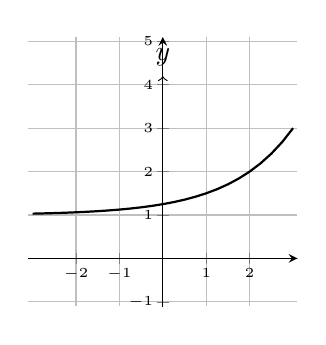
\begin{tikzpicture}%[domain=-4:4]
    \begin{axis}[
    grid=major,
    axis x line = middle,
    axis y line = middle,
        yticklabel style = {font=\tiny,xshift=0.5ex},
        xticklabel style = {font=\tiny,yshift=0.5ex},
    %scale only axis=true,
    width=5 cm,
    height=5 cm,
    xtick={-2,-1,0,1,2},
    ytick={-2,-1,0,1,2,3,4,5},
    xmin=-3.1,
    xmax=3.1,
    ymin=-1.1,
    ymax=5.1,
    ]
  %\draw[very thin,color=gray] (-2.9,-2.1) grid (2.9,2.9);

  \draw[->] (-4.2,0) -- (4.2,0) node[right] {$x$};
  \draw[->] (0,-1.2) -- (0,4.2) node[above] {$y$};

  \draw[thick, domain=-3:3]    plot (\x,1+.25*2^\x) ;%            node[right] {$f(x) =x$};
  % \x r means to convert '\x' from degrees to _r_adians:
  %\draw[thick, domain=-1:2]   plot (\x,2*\x) ;%   node[right] {$f(x) = \sin x$};
  %\draw[color=orange] plot (\x,{0.05*exp(\x)}) node[right] {$f(x) = \frac{1}{20} \mathrm e^x$};
  \end{axis}
\end{tikzpicture}

\choice \phantom{d}\vspace{-.7cm}
    
    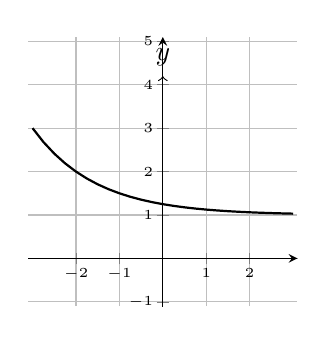
\begin{tikzpicture}%[domain=-4:4]
    \begin{axis}[
    grid=major,
    axis x line = middle,
    axis y line = middle,
        yticklabel style = {font=\tiny,xshift=0.5ex},
        xticklabel style = {font=\tiny,yshift=0.5ex},
    %scale only axis=true,
    width=5 cm,
    height=5 cm,
    xtick={-2,-1,0,1,2},
    ytick={-2,-1,0,1,2,3,4,5},
    xmin=-3.1,
    xmax=3.1,
    ymin=-1.1,
    ymax=5.1,
    ]
  %\draw[very thin,color=gray] (-2.9,-2.1) grid (2.9,2.9);

  \draw[->] (-4.2,0) -- (4.2,0) node[right] {$x$};
  \draw[->] (0,-1.2) -- (0,4.2) node[above] {$y$};

  \draw[thick, domain=-3:3]    plot (\x,1+.25*0.5^\x) ;%            node[right] {$f(x) =x$};
  % \x r means to convert '\x' from degrees to _r_adians:
  %\draw[thick, domain=-1:2]   plot (\x,2*\x) ;%   node[right] {$f(x) = \sin x$};
  %\draw[color=orange] plot (\x,{0.05*exp(\x)}) node[right] {$f(x) = \frac{1}{20} \mathrm e^x$};
  \end{axis}
\end{tikzpicture}

\end{checkboxes}
\end{multicols}

\question[4] \underline{Select all} of the functions graphed below which would have an inverse function.
\begin{multicols}{2}
    

\begin{checkboxes}
    \choice \phantom{a}\vspace{-.7cm}
    
    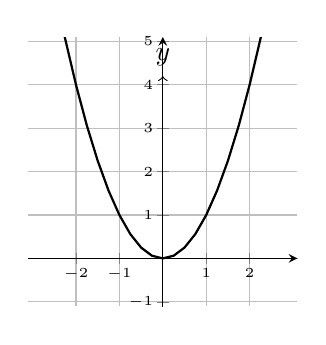
\begin{tikzpicture}%[domain=-4:4]
    \begin{axis}[
    grid=major,
    axis x line = middle,
    axis y line = middle,
        yticklabel style = {font=\tiny,xshift=0.5ex},
        xticklabel style = {font=\tiny,yshift=0.5ex},
    %scale only axis=true,
    width=5 cm,
    height=5 cm,
    xtick={-2,-1,0,1,2},
    ytick={-2,-1,0,1,2,3,4,5},
    xmin=-3.1,
    xmax=3.1,
    ymin=-1.1,
    ymax=5.1,
    ]
  %\draw[very thin,color=gray] (-2.9,-2.1) grid (2.9,2.9);

  \draw[->] (-4.2,0) -- (4.2,0) node[right] {$x$};
  \draw[->] (0,-1.2) -- (0,4.2) node[above] {$y$};

  \draw[thick, domain=-3:3]    plot (\x,\x*\x) ;%            node[right] {$f(x) =x$};
  % \x r means to convert '\x' from degrees to _r_adians:
  %\draw[thick, domain=-1:2]   plot (\x,2*\x) ;%   node[right] {$f(x) = \sin x$};
  %\draw[color=orange] plot (\x,{0.05*exp(\x)}) node[right] {$f(x) = \frac{1}{20} \mathrm e^x$};
  \end{axis}
\end{tikzpicture}

\choice \phantom{b}\vspace{-.7cm}
    
    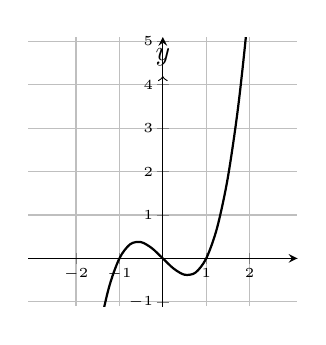
\begin{tikzpicture}%[domain=-4:4]
    \begin{axis}[
    grid=major,
    axis x line = middle,
    axis y line = middle,
        yticklabel style = {font=\tiny,xshift=0.5ex},
        xticklabel style = {font=\tiny,yshift=0.5ex},
    %scale only axis=true,
    width=5 cm,
    height=5 cm,
    xtick={-2,-1,0,1,2},
    ytick={-2,-1,0,1,2,3,4,5},
    xmin=-3.1,
    xmax=3.1,
    ymin=-1.1,
    ymax=5.1,
    ]
  %\draw[very thin,color=gray] (-2.9,-2.1) grid (2.9,2.9);

  \draw[->] (-4.2,0) -- (4.2,0) node[right] {$x$};
  \draw[->] (0,-1.2) -- (0,4.2) node[above] {$y$};

  \draw[thick, smooth, domain=-3:3]    plot (\x,\x*\x*\x-\x) ;%            node[right] {$f(x) =x$};
  % \x r means to convert '\x' from degrees to _r_adians:
  %\draw[thick, domain=-1:2]   plot (\x,2*\x) ;%   node[right] {$f(x) = \sin x$};
  %\draw[color=orange] plot (\x,{0.05*exp(\x)}) node[right] {$f(x) = \frac{1}{20} \mathrm e^x$};
  \end{axis}
\end{tikzpicture}

\choice \phantom{c}\vspace{-.7cm}
    
    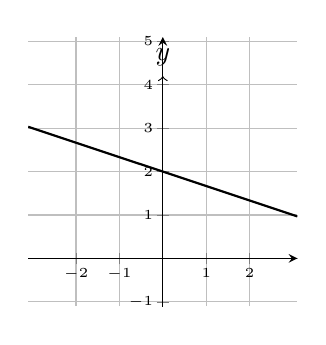
\begin{tikzpicture}%[domain=-4:4]
    \begin{axis}[
    grid=major,
    axis x line = middle,
    axis y line = middle,
        yticklabel style = {font=\tiny,xshift=0.5ex},
        xticklabel style = {font=\tiny,yshift=0.5ex},
    %scale only axis=true,
    width=5 cm,
    height=5 cm,
    xtick={-2,-1,0,1,2},
    ytick={-2,-1,0,1,2,3,4,5},
    xmin=-3.1,
    xmax=3.1,
    ymin=-1.1,
    ymax=5.1,
    ]
  %\draw[very thin,color=gray] (-2.9,-2.1) grid (2.9,2.9);

  \draw[->] (-4.2,0) -- (4.2,0) node[right] {$x$};
  \draw[->] (0,-1.2) -- (0,4.2) node[above] {$y$};

\draw[thick]
plot[variable=\t,domain=-3.1:3.1,smooth,thick] (\t, -0.333*\t+2);
  %\draw[thick, domain=-3:3]    plot (\x,1+.25*2^\x) ;%            node[right] {$f(x) =x$};
  % \x r means to convert '\x' from degrees to _r_adians:
  %\draw[thick, domain=-1:2]   plot (\x,2*\x) ;%   node[right] {$f(x) = \sin x$};
  %\draw[color=orange] plot (\x,{0.05*exp(\x)}) node[right] {$f(x) = \frac{1}{20} \mathrm e^x$};
  \end{axis}
\end{tikzpicture}

\choice \phantom{d}\vspace{-.7cm}
    
    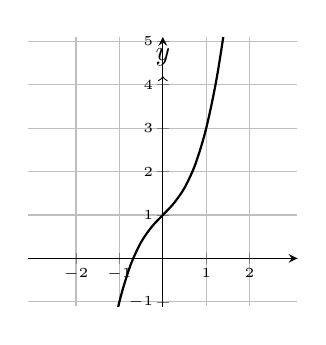
\begin{tikzpicture}%[domain=-4:4]
    \begin{axis}[
    grid=major,
    axis x line = middle,
    axis y line = middle,
        yticklabel style = {font=\tiny,xshift=0.5ex},
        xticklabel style = {font=\tiny,yshift=0.5ex},
    %scale only axis=true,
    width=5 cm,
    height=5 cm,
    xtick={-2,-1,0,1,2},
    ytick={-2,-1,0,1,2,3,4,5},
    xmin=-3.1,
    xmax=3.1,
    ymin=-1.1,
    ymax=5.1,
    ]
  %\draw[very thin,color=gray] (-2.9,-2.1) grid (2.9,2.9);

  \draw[->] (-4.2,0) -- (4.2,0) node[right] {$x$};
  \draw[->] (0,-1.2) -- (0,4.2) node[above] {$y$};

  \draw[thick, smooth, domain=-3:3]    plot (\x,\x*\x*\x+\x+1) ;%            node[right] {$f(x) =x$};
  % \x r means to convert '\x' from degrees to _r_adians:
  %\draw[thick, domain=-1:2]   plot (\x,2*\x) ;%   node[right] {$f(x) = \sin x$};
  %\draw[color=orange] plot (\x,{0.05*exp(\x)}) node[right] {$f(x) = \frac{1}{20} \mathrm e^x$};
  \end{axis}
\end{tikzpicture}

\end{checkboxes}
\end{multicols}

\newpage
\hspace{-.5in}Free answer section. Work must be shown to get credit for any answer. Partial credit may be given even for incorrect final answers, so show your work.



%\newpage

\question[10] %\textbf{[Section 2.6]} 
The graph of a function $y = f(x)$ is displayed below:

\includegraphics[scale=0.75]{Midterm2/transform.png}

Draw the graph of $y = 2f(-x) + 1$ below.

\includegraphics[scale=0.75]{Midterm2/transform_2.png}


\newpage

\question %\textbf{[Section 2.7]}
% \begin{parts}
%     \part
    [4] Given the graphs of functions $f(x)$ and $g(x)$ below, find $f\circ g(1)$.
    \begin{center}
    \includegraphics[scale=0.6]{Midterm2/composition.jpg}
    \end{center}
    \vspace{1cm}

    \question Let $f(x)=\frac{1}{x}+x$ and $g(x)=x^2+1$. 
    \begin{parts}
        \part[4] Find $f\circ g(x)$.
        \vspace{3cm}
        \part[4] Find $f\circ f(x)$.
    \newpage
 \end{parts}

\question %\textbf{[Section 2.8]}
Let $f(x)=\sqrt{x^3-1}$.

\begin{parts}
    \part[3] Find the domain of function $f(x)$.
    \vspace{4cm}
    \part[7] Find the inverse $f^{-1}(x)$.
    \vspace{7cm}
    % \part[3] Find the domain and range of the inverse function $f^{-1}(x)$.
\end{parts}

\newpage

\question %\textbf{[Section 3.1]} 
A manufacturer finds that the revenue generated by selling $x$ units of a certain commodity is given by the function 
\[
R(x) = 40 x - 5 x^2 \,. 
\]

\begin{parts}
    \part[6] Write the function $R(x)$ in vertex form.
    \vspace{8cm}

    \part[2] What is the maximum possible revenue generated?
    \vspace{3cm}

    \part[2] How many units should be manufactured to obtain the maximum revenue?
    \vspace{3cm}
\end{parts}

\newpage

\question %\textbf{[Section 3.2]} 
Let $f(x) = -3(x+1)(x-4)^3$ be a polynomial function.% which passes through the point $(x,y) = (2,-6)$.

\begin{parts}
%    \part[2] Find the value of $a$.
%    \vspace{3cm}
    \part[2] Fill in the blanks with the end behavior of $f(x)$.

    (No justification is needed.)
    \vspace{0.5cm}
    
    As $x \to \infty$, $y \to $ \rule{2cm}{0.15mm}.
    \vspace{0.5cm}
    
    As $x \to -\infty$, $y \to $ \rule{2cm}{0.15mm}.
    \vspace{0.5cm}
    \part[2] Find the $x$-intercepts (zeroes) of the function $f(x)$.
    \vspace{3cm}
    \part[6] Using part (b) and (c), sketch the graph of $f(x)$ on the $xy$-plane provided below. You need to clearly indicate the $x$-intercepts of $f(x)$ to receive full credit.
\begin{center}
\begin{figure}[H]
\centering
\begin{tikzpicture}[scale=1.5]
    \draw[->] (-4,0) -- (4,0) node[right] {$x$}; 
    \draw[->] (0,-2) -- (0,2) node[above] {$y$};
\end{tikzpicture}
\end{figure}
\end{center}
\end{parts}


\newpage
\question%[10] %\textbf{[Section 3.3]} 
Let $P(x)=5x^4+2x^2-x+1$ and $D(x)=x^2-x+2$. 

\begin{parts}
\part[7] Divide $P(x)$ by $D(x)$. 
\vspace{15cm}
\part[3] Express $P(x)$ in the form $D(x)\cdot Q(x)+R(x)$.


\end{parts}
\newpage
\question %\textbf{[Section 3.4]} 
Let $g(x) = 3x^{3}+7x^{2}-7x-3$.
\begin{parts}
\part[2] What are all the possible rational roots of $g(x)$ according to the rational root theorem?
\vspace{3cm}

\part[8] If we know that $g(x)$ has a root at $x=-3$, find all the roots of $g(x)$
\vspace{12cm}

\part[2] Write $g(x)$ as a product of linear factors.
\end{parts}


% \newpage
% \question %\textbf{[Section 4.1]} 
% Suppose two different laboratories, Lab A and Lab B, are running an experiment on colonies of bacteria.

% \begin{parts}
% \vspace{1cm}

% \part[4] At the start, Lab A has 100 bacteria colonies. Every day, the number of colonies doubles. How many bacteria colonies does Lab A have on day 4?


% \vspace{3cm}

% \part[4] Similarly, Lab B starts with 10 bacteria colonies. Every day, the number of colonies quadruples (e.g. is four times bigger each day). Write a function that described the number of colonies in Lab B on day number $n$.

% \vspace{3cm}

% \part[2] Suppose the experiment runs for several weeks. Which lab will have more bacteria colonies by the end and how do you know?

% \end{parts}
\newpage
\question For this problem, leave your answers in terms of an exponential. (Please do not try to expand the exponential or calculate the final values.)

Suppose you invest \$10,000 in a fund with 6\% annual interest.  Write an expression for the amount of money in the account after 5 years if interest is compounded:
\begin{parts}
\part[5] Quarterly ($n=4$ times per year)

\vspace{.4\textheight}

\part[5] Continuously% ($n = \infty$)
\end{parts}

\end{questions}